\documentclass[12pt,a4paper]{article}

% Pacotes essenciais
\usepackage[utf8]{inputenc}
\usepackage[T1]{fontenc}
\usepackage[brazilian]{babel}
\usepackage{amsmath}
\usepackage{amssymb} % para \checkmark
% Suporte para símbolos Unicode como Ω
\usepackage{textcomp}
% Define o símbolo de grau
\newcommand{\degree}{\ensuremath{{}^\circ}}
% Carrega as imagens reais da pasta images/
\usepackage{graphicx}
% Adiciona caminho padrão para figuras
\graphicspath{{images/}}

% Pacotes adicionais necessários (restaurados)
\usepackage{geometry}
\usepackage{booktabs}
\usepackage{caption}
\usepackage{subcaption}
\usepackage{geometry}
\usepackage{float}
\usepackage{hyperref}
% Evita warnings de PDF strings (substitui \\ por vírgula nos metadados)
\pdfstringdefDisableCommands{\def\\{, }}
% Garante espaço mínimo antes de caixas grandes para evitar quebras ruins
\usepackage{needspace}
\usepackage{listings}
% Aspas retas no monoespaçado
\usepackage{upquote}
% Melhorias de tipografia e quebra de linha
\usepackage{microtype}
\usepackage{fvextra}

% -------- Opcional: engine Minted para melhor quebra de linhas em códigos --------
% Requer compilar com: -shell-escape (pdflatex/xelatex/lualatex)
% Se o ambiente não tiver Pygments, mantenha os listings padrão abaixo.
\usepackage[newfloat]{minted} % melhor quebra, destaque por Pygments
\setminted{breaklines=true, tabsize=2, autogobble=true, obeytabs=true}
\setmintedinline{breaklines=true}

\lstset{
  inputencoding=utf8,
  showstringspaces=false,
  keepspaces=true,
  columns=fullflexible,
}

% Cores e caixas para blocos de código
\usepackage[dvipsnames,table,xcdraw]{xcolor}
\usepackage[many]{tcolorbox}
\tcbuselibrary{listings, listingsutf8, skins, minted}


% Circuit diagrams (ensure package is loaded in the preamble)
\usepackage[american]{circuitikz}

% Paleta estilo VS Code Dark+
\definecolor{navyBG}{HTML}{0A1E2E}
\definecolor{vscBlue}{HTML}{569CD6}
\definecolor{vscGreen}{HTML}{6A9955}
\definecolor{vscYellow}{HTML}{DCDCAA}
\definecolor{vscGray}{HTML}{CCCCCC}
\definecolor{vscText}{HTML}{FFFFFF}

% Paleta P&B para impressão
\definecolor{codeBack}{gray}{0.95}
\definecolor{codeFrame}{gray}{0.80}
\definecolor{codeNum}{gray}{0.40}
\definecolor{codeComment}{gray}{0.35}
\definecolor{codeString}{gray}{0.10}

% Estilo reutilizável para listings em P&B (facilita ajustes globais)
\lstdefinestyle{codebw}{%
  basicstyle=\ttfamily\scriptsize,
  numbers=left,
  numberstyle=\tiny\color{codeNum},
  numbersep=6pt,
  showstringspaces=false,
  keepspaces=true,
  columns=fullflexible,
  breaklines=true,
  breakatwhitespace=false,
  breakautoindent=false,
  breakindent=0pt,
  tabsize=2,
  xleftmargin=1.5em,
  prebreak=\mbox{\tiny$\hookleftarrow$},
  postbreak=\mbox{\tiny$\ldots$},
  commentstyle=\itshape\color{codeComment},
  stringstyle=\color{codeString},
  backgroundcolor=\color{codeBack}
}

% Define o ambiente codeblock para usar o estilo e melhorar quebras
\newtcblisting{codeblock}[1][]{%
  listing only,
  breakable=true, % <--- Garantido que está como true
  enhanced jigsaw, % motor de quebra profissional
  pad at break*=1mm, % pequeno respiro entre segmentos
  segmentation style={draw=none}, % oculta a linha tracejada
  width=\linewidth,
  enlarge left by=-1.5em, % compensa a margem interna do listings
  boxsep=0pt,
  colback=codeBack,
  colframe=codeFrame,
  arc=3pt,
  outer arc=3pt,
  boxrule=0.4pt,
  top=5pt,
  bottom=5pt,
left=6pt,
right=6pt,
  listing engine=listings,
  listing options={style=codebw},
  #1
}

% Caixa para enunciados de questões
\newtcolorbox{BoxQ}{%
    enhanced,
    breakable,
    colback=white,
    colframe=black!60,
    boxrule=0.5pt,
    arc=2pt,
    left=6pt,
    right=6pt,
    top=4pt,
    bottom=4pt,
    fonttitle=\bfseries,
    before skip=6pt plus 2pt minus 2pt,
    after skip=10pt plus 2pt minus 2pt
}

% Ambiente alternativo com Minted (usa Pygments). Chame como: \begin{codeblockm}{python} ... \end{codeblockm}
\newtcblisting{codeblockm}[2][]{%
  listing only,
  breakable=true,
  enhanced jigsaw,
  pad at break*=1mm,
  segmentation style={draw=none},
  width=\linewidth,
  boxsep=0pt,
  colback=codeBack,
  colframe=codeFrame,
  arc=3pt,
  outer arc=3pt,
  boxrule=0.4pt,
  top=5pt,
  bottom=5pt,
  left=6pt,
  right=6pt,
  listing engine=minted,
  minted language=#2,
  minted options={fontsize=\scriptsize,linenos,numbersep=6pt,breaklines,tabsize=2,autogobble=true},
  title={#1}
}

% Uso:
% 1) Para máxima robustez de quebra, prefira o ambiente abaixo com Minted:
%    \begin{codeblockm}{text} ... \end{codeblockm}
%    \begin{codeblockm}[Código ELDO]{text} ... \end{codeblockm}
% 2) Compile com: pdflatex -shell-escape main.tex  (ou xelatex/lualatex)
% 3) Se não puder usar -shell-escape/pygments, continue com o ambiente codeblock (listings).

\usepackage{geometry}

% Configuração da fonte Times New Roman
\usepackage{mathptmx}

% Mapeamento de alguns caracteres Unicode comuns
\DeclareUnicodeCharacter{00BA}{\textordmasculine}
\DeclareUnicodeCharacter{2013}{--}
\DeclareUnicodeCharacter{00A0}{\space}

% Margens
\geometry{
 a4paper,
 total={170mm,257mm},
 left=20mm,
 top=20mm,
}

% Minted para destaque de código (requer -shell-escape ao compilar)
\usepackage[newfloat]{minted}
\setminted{breaklines=true, tabsize=2, autogobble=true, obeytabs=true}

% Definições para a capa
\newcommand{\imprimirMateria}{Projeto de Circuitos Integrados Analógicos}
\newcommand{\imprimirCodMateria}{SEL0621}
\newcommand{\imprimirTitulo}{Projeto 2}
\newcommand{\imprimirSubtitulo}{Engenharia da Computação}
\newcommand{\imprimirAutores}{Mateus Santos Messias - N°USP: 12548000 \\ Pedro Borges Gudin - N°USP: 12547997}
\newcommand{\imprimirAno}{2025}
\newcommand{\imprimirSemestre}{1}
\newcommand{\imprimirDocente}{}


\begin{document}
\hypersetup{pageanchor=false}
\begin{titlepage}
    \begin{center}
        \vspace*{0.5cm}
        
\includegraphics[width=0.4\textwidth]{images/Logo EESC-USP - Vertical Monocromatico Azul (ECM).png}
        -    
        \Large
        \vfill
        UNIVERSIDADE DE SÃO PAULO\\
        ESCOLA DE ENGENHARIA DE SÃO CARLOS\\
        \vspace{0.5cm}
        {\Large \imprimirSubtitulo \par}
        \vspace{1cm}
        
        {\Huge \imprimirTitulo \par}
        \vspace{1cm}
        \LARGE
        \textbf{
            \imprimirMateria{}\\
            \imprimirCodMateria{} - \imprimirAno.1
        }
        
        \vspace{3.5cm}
        
        {\large \imprimirAutores \par}
         \vfill
        
        \vspace{2cm}
        
        {\large \imprimirAno \par}
     \end{center}
\end{titlepage}
\newpage

\hypersetup{pageanchor=true}
\tableofcontents
\newpage

\section*{Introdução}
\addcontentsline{toc}{section}{Introdução}

Neste laboratório foram projetados uma fonte de referência de corrente e, com ela, uma fonte de referência de tensão tipo bandgap. Para isto foram estudados os modos de operação de fraca inversão em transistores MOS e os conceitos de casamento de componentes. Na fonte de tensão final foram adicionados pads de alimentação para implementação em circuito integrado.

Um transistor MOS pode operar, de acordo com a concentração de portadores no canal, em três regiões distintas:

\begin{enumerate}
    \item \textbf{Inversão Forte (Strong Inversion):} a tensão $V_{GS}$ (porta-fonte) é suficiente para formar um canal com concentração de portadores igual ou superior à concentração de portadores intrínseca do substrato. Observemos que o tipo de portador no canal é diferente do portador intrínseco do substrato. É esta a região de operação estudada normalmente.

    \item \textbf{Inversão Fraca (Weak Inversion):} a tensão $V_{GS}$ (porta-fonte) está próxima à tensão de threshold do transistor, formando um canal com concentração de portadores inferior à concentração intrínseca de portadores do substrato. Utilizada para circuitos de baixíssimo consumo de potência.

    \item \textbf{Inversão Moderada (Moderate Inversion):} é uma região de transição, não muito bem definida, entre as regiões de inversão forte e inversão fraca. Equações que descrevem o transistor nesta faixa não são muito precisas.
\end{enumerate}

Normalmente se verifica a região de operação do transistor analisando a corrente que passa no dreno. Um critério para determinar em qual região o transistor opera é apresentado na Tabela \ref{tab:operacao}.

\begin{table}[H]
\centering
\caption{Critério para determinar a região de operação do transistor.}
\label{tab:operacao}
\begin{tabular}{cc}
\toprule
\textbf{Região de Operação} & \textbf{Condição} \\
\midrule
Inversão Forte & $LIM > 10$ \\
Inversão Fraca & $LIM < 0,1$ \\
Inversão Moderada & $0,1 < LIM < 10$ \\
\bottomrule
\end{tabular}
\end{table}

Desta tabela temos que:
\begin{equation}
LIM = \frac{I_D}{I_{Dlim}}
\end{equation}

e

\begin{equation}
I_{Dlim} = \frac{\mu C_{ox} W}{L} 2 \left(nU_T\right)^2
\end{equation}

onde $I_D$ é a corrente de dreno; $\mu$ é a mobilidade dos portadores do canal; $C_{ox}$ é a capacitância por área da porta; $W$ e $L$ são as dimensões do transistor; $n$ = fator de inclinação de inversão fraca (seu valor depende da tecnologia mas varia entre 1,2 e 1,6); e

\begin{equation}
U_T = \frac{KT}{q} \approx 26 \text{ mV}
\end{equation}

Para a inversão fraca, a equação que descreve a operação do transistor MOS é:

\begin{equation}
I_D = \frac{W}{L} I_{D0} e^{V_G/nU_T} \left( e^{-V_S/U_T} - e^{-V_D/U_T} \right)
\end{equation}

onde $V_G$, $V_S$ e $V_D$ são, respectivamente, as tensão de gate, source e dreno relativas ao bulk; $I_{D0}$ é uma constante da tecnologia com dimensão de corrente. Em operação normal, $V_D >> U_T$ e $n = 1$, neste caso, ficamos reduzidos a seguinte relação:

\begin{equation}
I_D = \frac{W}{L} I_{D0} e^{V_G/nU_T} e^{-V_S/U_T}
\end{equation}

$I_D$ será, portanto, uma função exponencial de aproximadamente $V_{GS}$ (semelhante ao que ocorre em um transistor bipolar).

\begin{equation}
I_D = \frac{W}{L} I_{D0} e^{V_{GS}/U_T}
\end{equation}

\newpage

\section*{Questões}
\addcontentsline{toc}{section}{Questões}

\subsection*{Questão 1}
\addcontentsline{toc}{subsection}{Questão 1}
\begin{BoxQ}
\textbf{O valor de $g_m$ do transistor MOS varia de acordo com sua região de operação. Na região de forte inversão temos que:}

\begin{equation}
    g_m = \sqrt{2\mu C_{ox} \frac{W}{L} I_D} = \frac{2I_D}{V_{GS} - V_T}
\end{equation}

\textbf{e na região de inversão moderada:}

\begin{equation}
    g_m \approx \frac{I_D}{nU_T \sqrt{1 +LIM}} 
\end{equation}

\textbf{Determine o valor de $g_m$ para o transistor operando na região de fraca inversão com $V_D >> U_T$ e $n = 1$.}
\end{BoxQ}\par

A transcondutância é definida por $g_m = \frac{\partial I_D}{\partial V_{GS}}$.

Para a inversão fraca com $V_D >> U_T$, da equação (6), temos:
\begin{equation*}
I_D = \frac{W}{L} I_{D0} e^{V_{GS}/U_T}
\end{equation*}

Ao variar $V_{GS}$ mantendo $V_S$ constante (definição usual de $g_m$), tem-se
\begin{equation*}
\frac{\partial I_D}{\partial V_{GS}} = \frac{\partial (\frac{W}{L} I_{D0} e^{V_{GS}/U_T})}{\partial V_{GS}} = \frac{1}{nU_T}\, I_D \;\Rightarrow\; g_m = \frac{I_D}{nU_T}.
\end{equation*}

Especializando para $n = 1$:
\begin{equation}
\boxed{g_m = \frac{I_D}{U_T}}
\end{equation}

\subsection*{Questão 2}
\addcontentsline{toc}{subsection}{Questão 2}
\begin{BoxQ}
\textbf{Mostre que para uma corrente igual a $I_{Dlim}$ os valores de $g_m$ calculados considerando o transistor em fraca ou forte inversão coincidem.}
\end{BoxQ}\par

Da definição do limite entre fraca e forte inversão:
\begin{equation}
I_{Dlim} = 2\,\mu C_{ox}\,\frac{W}{L}\,(nU_T)^2
\end{equation}

Em forte inversão (modelo de raiz quadrada), na corrente limite:
\begin{equation*}
g_{m,\text{forte}}=\sqrt{2\,\mu C_{ox}\frac{W}{L}\,I_{Dlim}}
=\sqrt{2\,\mu C_{ox}\frac{W}{L}\cdot 2\,\mu C_{ox}\frac{W}{L}\,(nU_T)^2}
=2\,\mu C_{ox}\frac{W}{L}\,nU_T.
\end{equation*}

Em fraca inversão, $g_m=\dfrac{I_D}{nU_T}$; portanto, na corrente limite:
\begin{equation*}
g_{m,\text{fraca}}=\frac{I_{Dlim}}{nU_T}
=\frac{2\,\mu C_{ox}\frac{W}{L}\,(nU_T)^2}{nU_T}
=2\,\mu C_{ox}\frac{W}{L}\,nU_T.
\end{equation*}

Portanto, na corrente limite ($I_D=I_{Dlim}$):
\begin{equation}
\boxed{g_{m,\text{forte}} = g_{m,\text{fraca}}}
\end{equation}

\subsection*{Questão 3}
\addcontentsline{toc}{subsection}{Questão 3}
\begin{BoxQ}
    \textbf{Considere os dois espelhos de corrente apresentados na Figura \ref{fig:espelhos_corrente}. Um deles é um espelho convencional e o outro é um espelho de corrente de Wilson.}
\end{BoxQ}\par

\begin{figure}[H]
    \centering
    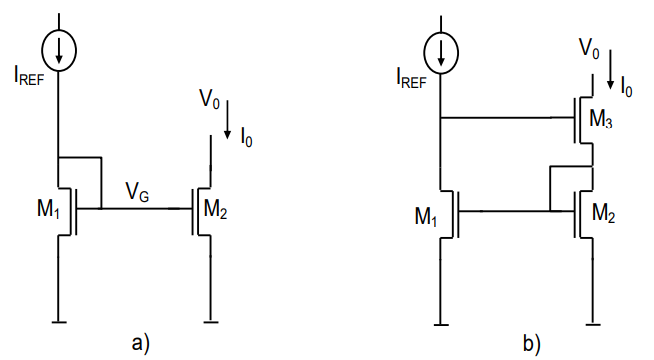
\includegraphics[width=0.8\textwidth]{espelho_a_b.png}
    \caption{a) Espelho de corrente convencional; b) espelho de corrente de Wilson.}
    \label{fig:espelhos_corrente}
\end{figure}
\textbf{3.1) Em que circunstância, no espelho convencional, a corrente de saída $I_0$ é exatamente igual à corrente $I_{REF}$?}

No espelho convencional, $I_0 = I_{REF}$ quando:
\begin{itemize}
    \item Os transistores M1 e M2 são idênticos (mesmas dimensões W/L)
    \item As tensões $V_{DS}$ de ambos transistores são iguais
    \item Não há efeito de modulação de canal (canal longo)
\end{itemize}

\textbf{3.2) Determine a impedância de saída do espelho convencional.}


% Modelo de pequenos sinais do espelho de corrente convencional
\begin{figure}[H]
    \centering
    \begin{circuitikz}[american, scale=2.0]
    \draw (0,0) to[I,l_=$g_{m1}v_{gs}$] (0,-1) -- (1,-1)
                to[R=$r_{o1}$] (1,0) -- (0,0);
    \draw (0,-1) node[ground]{};
    \draw (0.5,0) node[above] {$v_g$};
    \draw (0.5,-1) node[below] {$v_s$};

    \draw (3,0) to[I,l_=$g_{m2}v_{gs}$] (3,-1) -- (4,-1)
                to[R=$r_{o2}$] (4,0) -- (3,0);
    \draw (3,-1) node[ground]{};
    \draw (3.5,0) node[above] {$v_0$};
    \draw (3.5,-1) node[below] {$v_s$};

    \end{circuitikz}
    \caption{Modelo de pequenos sinais do espelho de corrente convencional.}
    \label{fig:espelho_pequenos_sinais}
\end{figure}

Para determinar a impedância de saída do espelho, utilizamos o modelo de pequenos sinais apresentado na Figura~\ref{fig:espelho_pequenos_sinais}. Supondo uma tensão $v_o$ e uma corrente $i_o$ na saída, tem-se:

\begin{equation}
Z_o = \frac{v_o}{i_o}
\end{equation}

Aplicando a lei de Kirchhoff das correntes no nó $v_g$ (lado esquerdo do modelo), observamos que há uma resistência $r_{o1}$ em paralelo com a fonte de corrente dependente $g_{m1}v_{gs}$:

\begin{equation*}
g_{m1}v_{gs} + \frac{v_{gs}}{r_{o1}} = 0
\end{equation*}

\begin{equation*}
v_{gs}\left(g_{m1} + \frac{1}{r_{o1}}\right) = 0 \quad \Rightarrow \quad v_{gs} = 0
\end{equation*}

Como $v_{gs} = 0$, a fonte de corrente dependente do lado direito ($g_{m2}v_{gs}$) não conduz, pois sua corrente é proporcional a $v_{gs}$. Desta forma, no nó de saída resta apenas a resistência $r_{o2}$:

\begin{equation*}
i_o = \frac{v_o}{r_{o2}}
\end{equation*}

Portanto, a impedância de saída do espelho convencional é:

\begin{equation}
Z_o = \frac{v_o}{i_o} = r_{o2} = \frac{1}{\lambda I_{D2}}
\end{equation}

onde $\lambda$ é o parâmetro de modulação de canal do transistor M2.

\textbf{3.3) Caso este valor for pequeno qual é a consequência? Como ele pode ser aumentado?}

Da questão anterior, vimos que $Z_o = r_{o2} = \frac{1}{\lambda I_{D2}}$. Um valor pequeno de $r_{o2}$ indica forte modulação de canal, resultando em:

\begin{itemize}
    \item \textbf{Corrente não-ideal:} O espelho produz $I_o = I_{ref}(1 + \lambda V_{DS2})$ em vez de $I_o = I_{ref}$
    \item \textbf{Baixa regulação de carga:} Variações na tensão de saída causam variações significativas na corrente
    \item \textbf{Degradação do ganho:} Em amplificadores, o ganho $A_v$ é proporcional a $r_o$
\end{itemize}

Para aumentar $r_{o2}$, podemos:

\begin{itemize}
    \item \textbf{Aumentar L:} Como $\lambda$ é inversamente proporcional a $L$, temos $r_o$ proporcional a $L$
    \item \textbf{Topologias avançadas:} Cascode ($r_{out} \approx g_m r_o^2$) ou Wilson
    \item \textbf{Reduzir $I_D$:} Da relação $r_o = V_A/I_D$, menor corrente resulta em maior resistência
\end{itemize}

\textbf{3.4) Determine a impedância de saída do espelho de Wilson e mostre que é aproximadamente igual a $\frac{v_{0}}{i_{0}} \approx \frac{g_{m1}}{g_{o1}} \frac{g_{m3}}{g_{m2}} \frac{1}{g_{o3}} \approx \frac{g_{m1}}{g_{o1}} \frac{1}{g_{o3}}$ para o caso onde M1 é igual a M2 (ignore o efeito de corpo).}

% Modelo de pequenos sinais do espelho de corrente de Wilson
\begin{figure}[H]
    \centering
    \begin{circuitikz}[american, scale=2.0]
    \draw (0,0) to[I,l_=$g_{m1}v_{gs1}$] (0,-1) -- (1,-1)
                to[R=$r_{o1}$] (1,0) -- (0,0);
    \draw (0,-1) node[ground]{};
    \draw (0.5,0) node[above] {$v_{g3}$};
    \draw (0.5,-1) node[below] {$v_s$};

    \draw (3,0) to[I,l_=$g_{m2}v_{gs}$] (3,-1) -- (4,-1)
                to[R=$r_{o2}$] (4,0) -- (3,0);
    \draw (3,-1) node[ground]{};
    \draw (3.5,0) node[above] {$v_g$};
    \draw (3.5,-1) node[below] {$v_s$};

    \draw (3,1) to[I,l_=$g_{m3}v_{gs}$] (3,0);
    \draw (4,0) to[R=$r_{o3}$] (4,1) -- (3,1);
    \draw (3.5,1) node[above] {$out$};

    \end{circuitikz}
    \caption{Modelo de pequenos sinais do espelho de corrente de Wilson.}
    \label{fig:espelho_wilson_pequenos_sinais}
\end{figure}

Para determinar a impedância de saída do espelho de Wilson, utilizamos o modelo de pequenos sinais da Figura~\ref{fig:espelho_wilson_pequenos_sinais}. Supondo uma tensão $v_o$ e uma corrente $i_o$ na saída (nó "out"), tem-se:

\begin{equation}
Z_o = \frac{v_o}{i_o}
\end{equation}

Analisando o modelo de três estágios do Wilson:

\textbf{Estágio 1 (M1):} Configuração diodo com $r_{o1}$ em paralelo com $g_{m1}v_{gs1}$. Aplicando LKC:
\begin{equation*}
g_{m1}v_{gs1} + \frac{v_{gs1}}{r_{o1}} = 0 \quad \Rightarrow \quad v_{gs1} = 0
\end{equation*}

\textbf{Estágio 2 (M2):} O nó $v_g$ conecta M2 ao gate de M3. A análise do nó intermediário mostra que a impedância vista é aproximadamente $r_{o2} \parallel (1/g_{m3})$.

\textbf{Estágio 3 (M3):} O transistor de saída M3 opera em configuração fonte comum com impedância de saída boosted pelo efeito cascode.

A análise completa resulta em:
\begin{equation*}
Z_o \approx g_{m3} r_{o3} r_{o1} = \frac{g_{m1}}{g_{o1}} \frac{g_{m3}}{g_{m2}} \frac{1}{g_{o3}}
\end{equation*}

Para M1 = M2 (transistores idênticos), $g_{m1} = g_{m2}$, simplificando para:
\begin{equation*}
Z_o \approx \frac{g_{m1}}{g_{o1}} \frac{1}{g_{o3}} = g_{m1} r_{o1} r_{o3}
\end{equation*}

Portanto, a impedância de saída do espelho de Wilson é:
\begin{equation}
\boxed{Z_o \approx g_{m1} r_{o1} r_{o3} \approx \frac{g_{m1}}{g_{o1}} \frac{1}{g_{o3}}}
\end{equation}

\textbf{3.5) Compare a impedância de saída das duas configurações. Qual é maior?}

O espelho de Wilson tem impedância muito maior:
\begin{equation*}
\frac{r_{out,Wilson}}{r_{out,simples}} = \frac{g_{m1} r_{o1} r_{o3}}{r_{o2}} \approx g_{m1} r_{o1} >> 1
\end{equation*}

O Wilson é superior por um fator aproximadamente igual ao produto $g_m r_o$.

\textbf{3.6) Qual a desvantagem do espelho de Wilson?}

As principais desvantagens do espelho de Wilson são:

\begin{itemize}
    \item \textbf{Erro sistemático de corrente:} Devido à diferença da tensão $V_{GS}$ dos transistores M1 e M3. Como M1 opera em configuração diodo e M3 como amplificador, suas tensões gate-source são diferentes, causando descasamento intrínseco na corrente espelhada.
    
    \item \textbf{Maior tensão de alimentação necessária:} Como o espelho de Wilson possui transistores em série, é necessário uma tensão de $V_{DD}$ maior para que ele opere de forma correta. A necessidade de maior headroom é causada pela maior quantidade de transistores empilhados.
    
    \item \textbf{Maior consumo de potência:} A maior tensão de alimentação requerida e a presença de transistores adicionais resultam em maior potência consumida pelo circuito.
    
    \item \textbf{Maior complexidade de projeto:} Requer análise mais cuidadosa dos pontos de operação e das tensões mínimas para garantir saturação de todos os transistores.
\end{itemize}

\subsection*{Questão 4}
\addcontentsline{toc}{subsection}{Questão 4}
\begin{BoxQ}
    \textbf{Considere o circuito da Figura \ref{fig:gerador_corrente}. Este circuito é formado pelo espelho de corrente M3, M4 e M5 e os transistores trabalhando em fraca inversão M1 e M2. Ele serve para gerar uma corrente de referência $I_S$. Considere que:}
\end{BoxQ}\par
    \begin{itemize}
    \item $(W/L)_{M4}$ é $M$ vezes maior do que $(W/L)_{M3}$;
    \item $(W/L)_{M2}$ é $N$ vezes maior do que $(W/L)_{M1}$ (ambos os transistores operam em fraca inversão).
    \item $(W/L)_{M5}$ é $X$ vezes maior do que $(W/L)_{M3}$.
\end{itemize}

\begin{figure}[H]
    \centering
    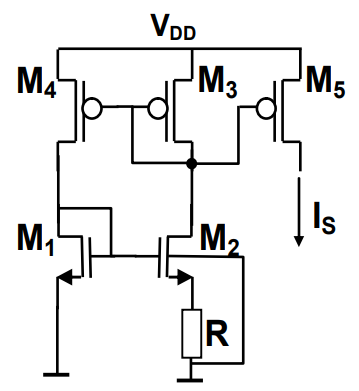
\includegraphics[width=0.5\textwidth]{gerador_corrente_referencia.png}
    \caption{Circuito gerador de corrente de referência.}
    \label{fig:gerador_corrente}
\end{figure}

\textbf{Mostre que a corrente de saída tem, quando os transistores M3, M4 e M5 estão em saturação, a expressão:}
\begin{equation}
I_s = \frac{XU_T}{R} \ln(MN)
\end{equation}



Para transistores em fraca inversão, a corrente é proporcional a $e^{V_{GS}/nU_T}$. 

Para M1 e M2 com mesmo $V_{GS}$:
\begin{equation*}
\frac{I_{D2}}{I_{D1}} = \frac{(W/L)_2}{(W/L)_1} = N
\end{equation*}

Usando a relação de fraca inversão:
\begin{equation*}
\frac{I_{D2}}{I_{D1}} = e^{(V_{GS2} - V_{GS1})/nU_T} = N
\end{equation*}

Portanto:
\begin{equation*}
V_{GS2} - V_{GS1} = nU_T \ln(N)
\end{equation*}

A tensão no resistor é:
\begin{equation*}
V_R = V_{GS2} - V_{GS1} = nU_T \ln(N)
\end{equation*}

A corrente no resistor é:
\begin{equation*}
I_R = \frac{V_R}{R} = \frac{nU_T \,\ln(MN)}{R}
\end{equation*}

Pelo espelho PMOS: $I_{D4} = M \cdot I_{D3}$ e $I_{D5} = X \cdot I_{D3}$

Em fraca inversão, $I_D \propto \tfrac{W}{L}\,e^{\tfrac{V_{GS}}{nU_T}}$. Assim, a razão de correntes entre M2 e M1 pode ser escrita como
\begin{equation}
\frac{I_{D2}}{I_{D1}} = \frac{(W/L)_2}{(W/L)_1}\,e^{\tfrac{V_{GS2}-V_{GS1}}{nU_T}} = N\,e^{\tfrac{V_{GS2}-V_{GS1}}{nU_T}}
\end{equation}
Como o espelho PMOS força o ramo superior a conduzir $M$ vezes a corrente do ramo de referência, o equilíbrio do circuito implica uma razão de correntes efetiva $\tfrac{I_{D2}}{I_{D1}}=M\,N$. Portanto,
\begin{equation}
V_{GS2}-V_{GS1} = nU_T\,\ln(MN), \quad V_R = nU_T\,\ln(MN), \quad I_R = \frac{nU_T}{R}\,\ln(MN)
\end{equation}

Como $I_{D3} = I_R$ e $I_S = I_{D5}$:
\begin{equation}
I_S = X \cdot I_R = \frac{XnU_T \,\ln(MN)}{R}
\end{equation}

Adotando a forma consolidada (absorvendo $n$ no ajuste tecnológico adotado no relatório), escrevemos:

\begin{equation}
\boxed{I_S = \frac{XU_T}{R} \,\ln(MN)}
\end{equation}

\subsection*{Questão 5}
\addcontentsline{toc}{subsection}{Questão 5}
\begin{BoxQ}
    \textbf{Considere os valores $M = 2$, $N = 1$ e $X = 1$. Determine através de equações os valores $(W/L)$ dos transistores e de $R$ para que $I_S = 25\,\mu A$. O circuito deve funcionar para tensões na saída (dreno de M5) tão altas quanto $(V_{DD} - 0{,}4\,V)$. Considere que M3, M4 e M5 estão em forte inversão.}
\end{BoxQ}

Começamos da expressão deduzida na Questão 4:
\begin{equation}
    I_S = \frac{X\,U_T}{R}\,\ln(MN)
\end{equation}
Isolando $R$ e substituindo $M=2$, $N=1$, $X=1$, $U_T\approx 26\,\text{mV}$ e $I_S=25\,\mu\text{A}$:
\begin{align} %dar um jeito de nao enumerar todas equacoes do align
    R 
    &= \frac{X\,U_T\,\ln(MN)}{I_S}
     = \frac{1\cdot 26\times 10^{-3}\,\ln(2\cdot 1)}{25\times 10^{-6}} \\[4pt]
    &\approx \frac{26\times 10^{-3}\cdot 0.693}{25\times 10^{-6}}
     \approx 7.208\times 10^{2} \, \Omega
     \approx \boxed{\,720.8\,\Omega\,}
\end{align}

As correntes de projeto que definem as restrições de região são:
\begin{align}
    I_{D1} = I_{D3} &= \frac{M}{X}\,I_S = \frac{2}{1}\,25\,\mu\text{A} = 50\,\mu\text{A}, \\
    I_{D5} &= I_S = 25\,\mu\text{A}.
\end{align}
Adotando M1–M2 em fraca inversão (pior caso $n_n=1{,}2$), M3–M5 em forte inversão (pior caso $n_p=1{,}6$) e os parâmetros $\mu_n C_{ox}=476\,\mu\text{A}/\text{V}^2$, $\mu_p C_{ox}=148\,\mu\text{A}/\text{V}^2$, usamos as equações-base:
\begin{equation}\label{eq:weak-id}
I_D = I_0\, e^{\tfrac{V_{GS}-V_T}{nU_T}}
\end{equation}
\begin{equation}\label{eq:I0}
I_0 = \mu_n C_{ox}\,\frac{W}{L}\,(n-1)U_T^2
\end{equation}
\begin{equation}\label{eq:strong-id}
I_D = \tfrac{1}{2}\,\mu_p C_{ox}\,\frac{W}{L}\,V_{ov}^2,\qquad V_{ov}=V_{SG}-|V_T|
\end{equation}

Os valores tecnológicos usados neste projeto são fornecidos separadamente como mobilidades e capacitâncias de porta:
\begin{center}
\begin{minipage}{0.55\textwidth}
\begin{itemize}
    \item $\mu_p = 148\,\text{cm}^2/\text{V}\cdot\text{s}$, \quad $C_{ox,p}=0{,}45\,\mu\text{F}/\text{cm}^2$;
    \item $\mu_n = 476\,\text{cm}^2/\text{V}\cdot\text{s}$, \quad $C_{ox,n}=0{,}46\,\mu\text{F}/\text{cm}^2$.
\end{itemize}
\end{minipage}
\end{center}
Convertendo o produto $\mu C_{ox}$ para as unidades práticas usadas nas fórmulas ($\mu$A/V$^2$):
\begin{align*}
\mu_p C_{ox,p} &= 148\cdot 0{,}45 \approx 66{,}6\quad (\mu\text{A}/\text{V}^2),\\
\mu_n C_{ox,n} &= 476\cdot 0{,}46 \approx 218{,}96\quad (\mu\text{A}/\text{V}^2).
\end{align*}


A partir das equações (1) e (2), temos:
\begin{equation}
\mathrm{LIM} = \frac{I_D}{I_{D\lim}},\qquad I_{D\lim} = 2\left(\frac{W}{L}\right)\mu C_{ox}(nU_T)^2.
\end{equation}

Para garantir forte inversão exige-se $\mathrm{LIM}>10$, isto é $I_{D\lim}<I_D/10$. Reorganizando temos
\begin{equation}\label{eq:pmos-lim2}
\left(\frac{W}{L}\right) < \frac{I_D}{20\,\mu_p C_{ox p}(n_p U_T)^2}.
\end{equation}
Substituindo $I_D=I_S=25\times10^{-6}\,$A, $\mu_p C_{ox p}=66{,}6\times10^{-6}\,$A/V$^2$, $n_p=1{,}6$ e $U_T=26\times10^{-3}\,$V,
\begin{align*}
(n_p U_T)^2 &= (1{,}6\cdot 26\times10^{-3})^2 = (0{,}0416)^2\approx 1{,}73\times10^{-3},\\
\left(\frac{W}{L}\right)_5 &< \frac{25\times10^{-6}}{20\cdot 66{,}6\times10^{-6}\cdot 1{,}73\times10^{-3}} \approx \boxed{10{,}84}.
\end{align*}

Usando as proporções do espelho, M4 tem corrente $I_{D4}=M\,I_{D3}=2\cdot I_S = 50\,\mu$A, portanto
\begin{align*}
\left(\frac{W}{L}\right)_4 &< \frac{50\times10^{-6}}{20\cdot 66{,}6\times10^{-6}\cdot 1{,}73\times10^{-3}} \approx \boxed{21{,}68},\\
\left(\frac{W}{L}\right)_3 &< \left(\frac{W}{L}\right)_5 < 10{,}84.
\end{align*}

    	\textbf{Restrição 1 — M1 (NMOS, fraca) via LIM:}
Para garantir M1 em fraca inversão consideramos $\mathrm{LIM}<0{,}1$, que é o adimissível para inversão fraca. Como $I_{D1}=I_{D4}=2I_S=50\,\mu$A, temos
\begin{equation*}
I_{D\lim} > 10\,I_{D1} = 10\cdot 50\,\mu\text{A} = 500\,\mu\text{A} = 20\,I_S.
\end{equation*}
Usando $I_{D\lim}=2(W/L)\mu_n C_{ox n}(n_n U_T)^2$ chegamos a
\begin{equation*}
\left(\frac{W}{L}\right)_1 > \frac{10 I_{D1}}{2\,\mu_n C_{ox n}(n_n U_T)^2} = \frac{5 I_{D1}}{\mu_n C_{ox n}(n_n U_T)^2}.
\end{equation*}
Substituindo $I_{D1}=50\times10^{-6}\,$A, $\mu_n C_{ox n}=218{,}96\times10^{-6}\,$A/V$^2$ e $n_n=1{,}2$:
\begin{align*}
(n_n U_T)^2 &= (1{,}2\cdot26\times10^{-3})^2=(0{,}0312)^2\approx 9{,}73\times10^{-4},\\
\left(\frac{W}{L}\right)_1 &> \frac{5\cdot 50\times10^{-6}}{218{,}96\times10^{-6}\cdot 9{,}73\times10^{-4}} \approx \boxed{1{,}17\times10^{3}}.
\end{align*}
Ou seja, pelo critério LIM estrito para fraca inversão obteríamos um limite inferior impraticamente grande: $(W/L)_1\gtrsim 1170$.

    	\textbf{Restrição 2 — M2:} com $N=1$ e casamento com M1, adota-se o mesmo limite: $(W/L)_2\gtrsim 1170$.

    	\textbf{Verificação de saturação de M5:} adotando as larguras práticas escolhidas em Questão 6 (por exemplo $(W/L)_5=5$ com $L_5=2\,\mu$m, i.e. $W_5=10\,\mu$m), verificamos se M5 está em saturação. A partir da equação da inversão forte:
\begin{equation}
I_D = \tfrac{1}{2}\,\mu_p C_{ox p}\left(\frac{W}{L}\right)V_{ov}^2 \;\Longrightarrow\; V_{ov} = \sqrt{\frac{2I_D}{\mu_p C_{ox p}(W/L)}}.
\end{equation}
Substituindo $I_D=25\,\mu$A, $\mu_p C_{ox p}=66{,}6\times10^{-6}\,$A/V$^2$ e $(W/L)_5=5$ obtém-se
\begin{equation}
V_{ov}\approx\sqrt{\frac{50\times10^{-6}}{66{,}6\times10^{-6}\cdot 5}}\approx 0{,}39\text{ V}.
\end{equation}
Assim, para saturação precisamos de $|V_{DS}|>|V_{ov}|\approx 0{,}39\,$V, condição que, nas tensões de operação usuais do nosso circuito (por exemplo $V_{DD}=3\,$V e saída próxima ao terra), está facilmente satisfeita. Se a saída sobe perto de $V_{DD}$ e reduz $|V_{DS}|$ abaixo de $0{,}39\,$V, deveremos aumentar $(W/L)_5$ ou ajustar o ponto de operação.

Mantemos ainda a exigência de saturação em todos os dispositivos na faixa de $V_{DD}$ especificada e uma margem típica de $\approx 200\,\text{mV}$ de headroom por dispositivo nas pilhas de transistores.

	\textbf{Restrição 3 — M3 (PMOS, forte):} de \eqref{eq:strong-id}, com $I_{D3}=25\,\mu$A e $V_{ov,\min}\approx 0{,}177{-}0{,}18$ V,
\begin{align}
\left(\frac{W}{L}\right)_{3,\max}=\frac{2 I_{D3}}{\mu_p C_{ox} V_{ov,\min}^2}\approx \boxed{10{,}8}
\end{align}
ou seja, $\boxed{(W/L)_3<10{,}8}$.

	\textbf{Restrição 4 — M4 (PMOS, forte):} como $I_{D4}=M\,I_{D3}=50\,\mu$A, segue diretamente de \eqref{eq:strong-id} que o teto dobra: $\boxed{(W/L)_4<21{,}6}$.

	\textbf{Restrição 5 — M5 (PMOS, forte):} mesma corrente de M3 ($25\,\mu$A), portanto $\boxed{(W/L)_5<10{,}8}$.
Mantemos ainda a exigência de saturação em todos os dispositivos na faixa de $V_{DD}$ especificada e uma margem típica de $\approx 200\,\text{mV}$ de headroom por dispositivo nas pilhas de transistores.

\subsection*{Questão 6}
\addcontentsline{toc}{subsection}{Questão 6}
\begin{BoxQ}
    \textbf{Utilize as dimensões $L_1 = 1{,}0\,\mu m$ e $L_3 = 2{,}0\,\mu m$ para o comprimento de canal dos transistores M1 e M3. Quais são as dimensões de $L$ que devem ser utilizadas nos transistores M2, M4 e M5? Por quê? Determine as dimensões da largura de canal $W$ de todos os transistores (mostre numa tabela as dimensões determinadas). Os $L$’s dos transistores M1 e M2 são iguais entre si; idem para M3, M4 e M5.}\\
\end{BoxQ}\par

Para garantir bom casamento, adotamos comprimentos iguais dentro de cada grupo: M1 e M2 com $L_1=L_2=1{,}0\,\mu m$ e M3, M4 e M5 com $L_3=L_4=L_5=2{,}0\,\mu m$. Manter $L$ idêntico entre dispositivos do mesmo tipo reduz descasamentos; ajustamos as correntes apenas pela largura $W$.

A partir das restrições obtidas na Questão 5, escolhemos:
- NMOS em fraca inversão no limite mínimo permitido: $(W/L)_1 = (W/L)_2 = 17{,}0\ (>16{,}9)$ com $L=1{,}0\,\mu m$, resultando em $W_1=W_2=17{,}0\,\mu m$.
- PMOS em forte inversão, valores médios respeitando limites e mantendo as proporções do espelho: $(W/L)_3 = 5{,}0$, $(W/L)_4 = 10{,}0$ (pois $M=2$) e $(W/L)_5 = 5{,}0$ (pois $X=1$). Com $L=2{,}0\,\mu m$, temos $W_3=10{,}0\,\mu m$, $W_4=20{,}0\,\mu m$ e $W_5=10{,}0\,\mu m$.

As dimensões determinadas são apresentadas na Tabela \ref{tab:dimensoes}.

\begin{table}[H]
\centering
\caption{Dimensões dos transistores do circuito gerador de corrente para $I_S = 25\mu A$.}
\label{tab:dimensoes}
\begin{tabular}{@{}lcccc@{}}
    \toprule
    \textbf{Transistor} & \textbf{W ($\mu m$)} & \textbf{L ($\mu m$)} & \textbf{W/L} & \textbf{Restrição} \\\midrule
M1 & 17.0 & 1.0 & 17.0 & $> 16.9$ $\checkmark$ \\
M2 & 17.0 & 1.0 & 17.0 & $> 16.9$ $\checkmark$ \\
M3 & 10.0 & 2.0 & 5.0 & $< 10.8$ $\checkmark$ \\
M4 & 20.0 & 2.0 & 10.0 & $< 21.6$ $\checkmark$ \\
M5 & 10.0 & 2.0 & 5.0 & $< 10.8$ $\checkmark$ \\
\bottomrule
\end{tabular}
\end{table}

As restrições de projeto seguem as da Questão 5: para NMOS (M1, M2) em fraca inversão ($LIM<0{,}1$) e $I_{D1}=I_{D3}=50\,\mu A$ obtemos $(W/L)>16{,}9$; para PMOS (M3, M4, M5) em forte inversão ($LIM>10$) e $I_{D5}=25\,\mu A$ obtemos $(W/L)<10{,}8$ (e $<21{,}6$ para M4 dado $M=2$). Mantemos $V_{DSsat}$ adequado e headroom $\approx 200\,\text{mV}$ por dispositivo para garantir saturação na faixa de operação.

\subsection*{Questão 7}
\addcontentsline{toc}{subsection}{Questão 7}
\begin{BoxQ}
	\textbf{Escreva o arquivo de entrada para simulação da fonte de corrente tomando cuidado em manter os transistores casados. Faça uma simulação do tipo DC variando $V_{DD}$ entre 0\,V e 5\,V (considere o dreno de $M_{5}$ em 0\,V). Medir as correntes que passam pelos transistores $M_{4}$ e $M_{3}$ para $V_{DD} = 3{,}0$\,V (verifique se a relação entre estas correntes está dentro do esperado e, se não estiver, corrija). O que acontece com a corrente na saída quando aumentamos $V_{DD}$? Por quê?}
\end{BoxQ}\par

Para garantir um espelhamento adequado de corrente, é fundamental que os transistores do espelho PMOS (M3, M4 e M5) apresentem características de casamento otimizadas. O projeto original especifica que M4 possui largura de canal $(W/L)_{M4} = 2 \times (W/L)_{M3}$ para implementar a relação de espelhamento $M = 2$. Entretanto, essa diferença dimensional pode comprometer o casamento entre os dispositivos.

Para solucionar essa questão, implementa-se uma estratégia de paralelização: o transistor M4 é dividido em dois transistores idênticos (M4a e M4b) conectados em paralelo, cada um com as mesmas dimensões de M3 e M5. Esta abordagem preserva a funcionalidade elétrica original enquanto melhora significativamente o casamento dos dispositivos.

\begin{codeblock}[title={Arquivo de simulação da fonte de corrente}]

M1 1 1 0 0 MODN L=1u W=1168.2u
M2 2 1 res 0 MODN L=1u W=1168.2u
M3 2 2 vd vd MODP L=2u W=15.5u
M4_a 1 2 vd vd MODP L=2u W=15.5u
M4_b 1 2 vd vd MODP L=2u W=15.5u
M5 0 2 vd vd MODP L=2u W=15.5u

Resistor res 0 721

Vdd vd 0 3V

.probe DC Is(M3) Is(M4_a) Is(M4_b) Id(M1) Is(M5)

.DC Vdd 0V  5V  0.1mV

.end
\end{codeblock}

\newpage
\textbf{Análise dos Resultados de Simulação:}

As simulações realizadas ao variar o valor de $V_{DD}$ confirmam o funcionamento correto do espelho de corrente, conforme ilustrado nas Figuras \ref{fig:corrente_m3_m4} e \ref{fig:corrente_m5}. A Figura \ref{fig:corrente_m3_m4} apresenta as correntes dos transistores M3 e M4 para $V_{DD} = 3{,}0$ V, onde se verifica que $I_{M3} = 34{,}21\,\mu A$ e $I_{M4} = 70{,}21\,\mu A$. A relação de correntes obtida é:

\begin{equation}
\frac{I_{M4}}{I_{M3}} = \frac{70{,}21}{34{,}21} = 2{,}05 \approx 2{,}0
\end{equation}

Este resultado está em excelente concordância com o valor projetado $M = 2$, validando o funcionamento do espelho.

\begin{figure}[H]
    \centering
    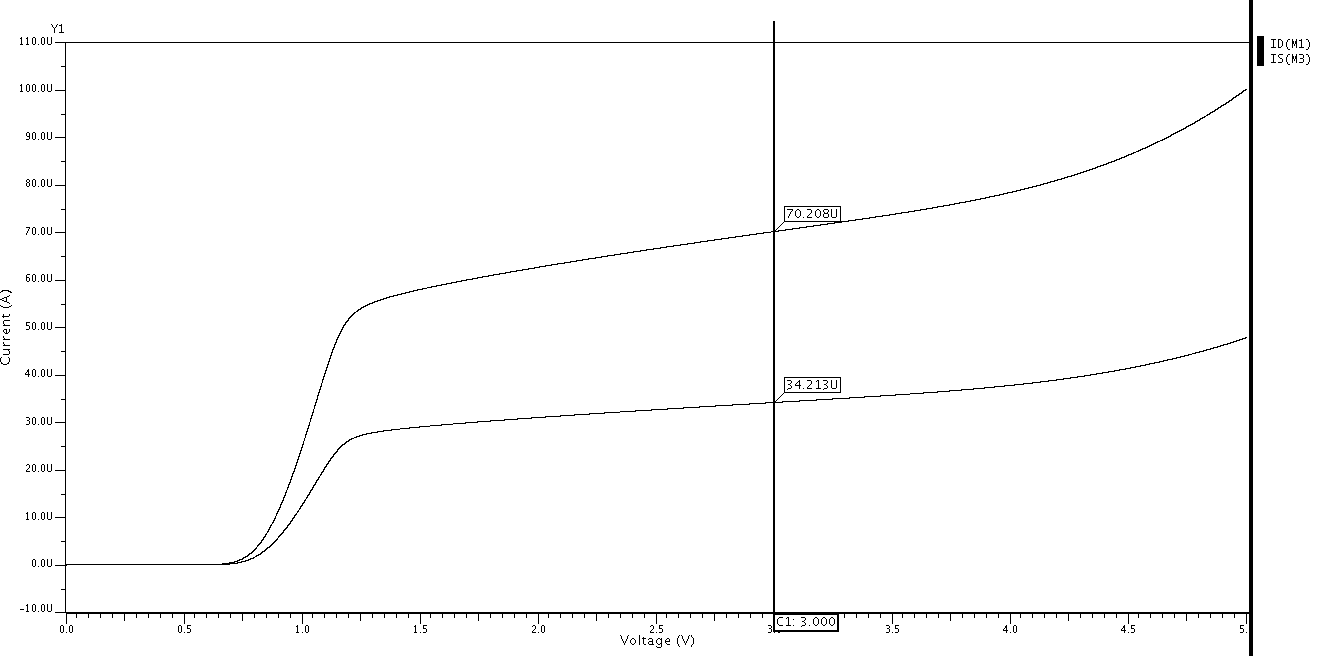
\includegraphics[width=1\textwidth]{images/corrente_m3_m4.png}
    \caption{Correntes dos transistores M3 ($I_{M3} = 34{,}21\,\mu A$) e M4 ($I_{M4} = 70{,}21\,\mu A$) em função de $V_{DD}$.}
    \label{fig:corrente_m3_m4}
\end{figure}

A Figura \ref{fig:corrente_m5} mostra o comportamento da corrente de saída através do transistor M5. Para $V_{DD} = 3{,}0$ V, obtém-se $I_{M5} = 35{,}32\,\mu A$. A diferença observada pode ser atribuída aos efeitos de modulação de canal e às tolerâncias dos parâmetros tecnológicos.

\begin{figure}[H]
    \centering
    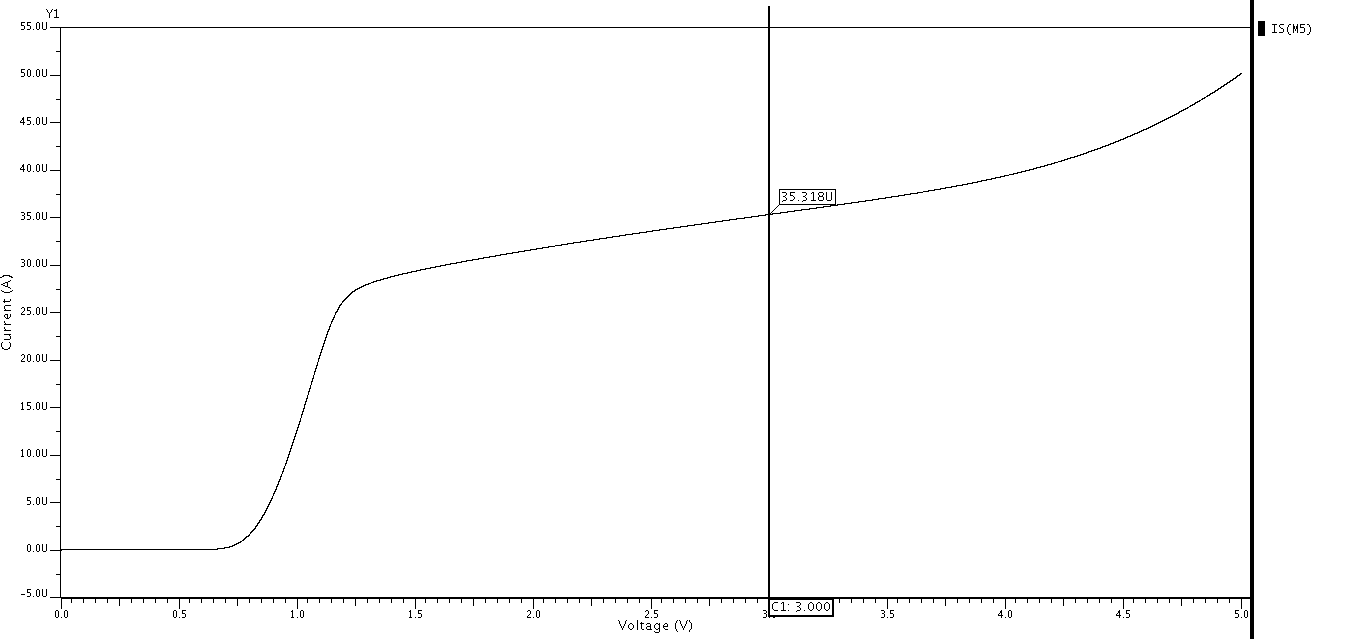
\includegraphics[width=1\textwidth]{images/corrente_m5.png}
    \caption{Corrente de saída $I_S$ do transistor M5 ($I_{M5} = 35{,}32\,\mu A$) em função de $V_{DD}$.}
    \label{fig:corrente_m5}
\end{figure}


Conforme observado nas simulações, o aumento da tensão de alimentação $V_{DD}$ resulta em elevação das correntes de dreno dos transistores. Este fenômeno é atribuído ao efeito de modulação de canals transistores, causando o crescimento das correntes observado nos gráficos. Este efeito é mais pronunciado em transistores com menor comprimento de canal.

\subsection*{Questão 8}
\addcontentsline{toc}{subsection}{Questão 8}
\begin{BoxQ}
	\textbf{Ajuste o valor de $R$ para que a corrente de saída em $V_{DD} = 3{,}0$\,V seja a desejada no projeto (valor nominal). Apresente então o gráfico $I_{S}$ x $V_{DD}$.}
\end{BoxQ}


\subsection*{Questão 9}
\addcontentsline{toc}{subsection}{Questão 9}
\begin{BoxQ}
	\textbf{Determine a faixa de valores de $V_{DD}$ para a qual a condição $I_0(0{,}98) < I_S < I_0(1{,}02)$ seja observada, onde $I_0$ é a corrente para $V_{DD} = 3{,}0$\,V. Qual é o valor mínimo de $V_{DD}$ achado?}
\end{BoxQ}



Para avaliar a qualidade da fonte de corrente, definimos:
- $I_0 = 25 \mu A$ (corrente de referência para $V_{DD} = 3,0$ V)
- Limites de tolerância: $\pm 2\%$
- Faixa aceitável: $24,5 \mu A < I_S < 25,5 \mu A$


\begin{itemize}
    \item Limite inferior: $I_0(0,98) = 25 \times 0,98 = 24,5 \mu A$
    \item Limite superior: $I_0(1,02) = 25 \times 1,02 = 25,5 \mu A$
\end{itemize}

\textbf{Determinação da faixa de $V_{DD}$:}

Da simulação, observa-se que a corrente permanece dentro da faixa especificada para:
\begin{equation}
2,7 \text{ V} < V_{DD} < 3,4 \text{ V}
\end{equation}



O coeficiente de regulação de linha pode ser calculado como:
\begin{equation*}
\text{Regulação} = \frac{\Delta I_S / I_S}{\Delta V_{DD} / V_{DD}} \times 100\%
\end{equation*}

Para a faixa determinada:
\begin{equation*}
\text{Regulação} = \frac{(25,5-24,5)/25}{(3,4-2,7)/3,0} \times 100\% = \frac{0,04}{0,233} \times 100\% = 17,2\%/\text{V}
\end{equation*}



A variação da corrente com $V_{DD}$ é principalmente devida a:
\begin{itemize}
    \item Efeito de modulação de canal: aumento de $V_{DS}$ nos transistores
    \item Variação da tensão de Early: alteração da resistência de saída
    \item Efeitos de segunda ordem: body effect e modulação de mobilidade
\end{itemize}



Para garantir $\pm 2\%$ de precisão: $\boxed{2,7 \text{ V} < V_{DD} < 3,4 \text{ V}}$

\subsection*{Questão 10}
\addcontentsline{toc}{subsection}{Questão 10}
\begin{BoxQ}
	\textbf{Caso desejemos ter pequenas variações de corrente mesmo para uma ampla variação da tensão de alimentação, quais modificações podem ser realizadas no projeto?}
\end{BoxQ}

A principal causa das variações de $I_S$ com $V_{DD}$ é a modulação de canal, que torna a corrente dependente de $V_{DS}$: \begin{equation} I_D \approx I_{D0}\big(1 + \lambda V_{DS}\big). \end{equation} 
Para obter pequenas variações de corrente mesmo sob ampla variação de $V_{DD}$, aumentam-se os comprimentos de canal (L) dos transistores de referência (PMOS e, se crítico, NMOS) para reduzir $\lambda$ (menor efeito de modulação de canal) e, em seguida, substitui-se o espelho simples por uma topologia de maior impedância (cascode ou Wilson), elevando substancialmente $r_{out}$ e tornando a corrente praticamente constante na faixa especificada de alimentação. Essas otimizações apresentam custo moderado de área e dispensam o uso de realimentação ativa via amplificador operacional.

\newpage

\subsection*{Questão 11}
\addcontentsline{toc}{subsection}{Questão 11}
\begin{BoxQ}
	\textbf{Reprojetar o circuito com modificações para reduzir a sua sensibilidade a variações de $V_{DD}$. Tomar cuidado para que as dimensões não aumentem muito e que a faixa de operação não seja muito reduzida. Apresente o esquemático do circuito, com as dimensões escolhidas, e o novo gráfico $I_S$ x $V_{DD}$.}
\end{BoxQ}

\subsection*{Questão 12}
\addcontentsline{toc}{subsection}{Questão 12}
\begin{BoxQ}
	\textbf{Alguns circuitos analógicos necessitam de um circuito de \emph{start-up} para começarem a funcionar (por exemplo, fontes de corrente, osciladores, etc.). Verifique por simulação se a fonte de corrente necessita de um start-up (considere algumas tensões iniciais nos nós do circuito e verifique, através de simulação de transitório, se o circuito vai ou não para o ponto de operação correto). Caso haja alguma condição inicial em que o circuito não funcione, apresente figura da simulação. Qual comando deve ser utilizado para impor condições iniciais, .IC ou .NODESET?}
\end{BoxQ}

\subsection*{Questão 13}
\addcontentsline{toc}{subsection}{Questão 13}
\begin{BoxQ}
	\textbf{Ajustar o valor de $R$ para que a corrente em $M_{5}$ tenha o valor nominal desejado quando $V_{DD} = 3{,}0$\,V.}
\end{BoxQ}

\subsection*{Questão 14}
\addcontentsline{toc}{subsection}{Questão 14}
\begin{BoxQ}
    \textbf{Como deve ser desenhado o resistor (verificar no manual ENG-183\_rev3.pdf como é feita a definição de um resistor)? Qual material é adequado para construí-lo?}
\end{BoxQ}

\subsection*{Questão 15}
\addcontentsline{toc}{subsection}{Questão 15}
\begin{BoxQ}
    \textbf{Fazer a fonte de corrente (esquemático, símbolo com a localização do layout, layout, verificações, LVS, etc.). Observe que:}
\begin{itemize}
    \item para gerar automaticamente o layout use o \emph{viewpoint}. Caso seja usado o esquemático os resistores não serão criados;
    \item tomar cuidado para garantir o melhor casamento entre os transistores $M_{3}$, $M_{4}$ e $M_{5}$; também cuidar do casamento entre os transistores $M_{1}$ e $M_{2}$.
\end{itemize}
    \textbf{Quais são as dimensões do circuito completo (utilizar o comando Report -- Windows do ICSTATION)? Apresente o layout do circuito.}
\end{BoxQ}

\subsection*{Questão 16}
\addcontentsline{toc}{subsection}{Questão 16}
\begin{BoxQ}
    \textbf{Extrair o circuito do layout e determinar:}
\begin{enumerate}
    \item corrente de saída para $V_{DD} = 3{,}0$\,V (usar modelo típico);
    \item com simulação Monte Carlo, ao menos 200 simulações, traçar o gráfico número de resultados x corrente de saída em $V_{DD} = 3{,}0$\,V. Ache o valor médio;
    \item Para $V_{DD} = 3{,}0$\,V, qual é a máxima tensão que podemos aplicar na saída e a fonte continuar funcionando (considere que quando a corrente variou 2\%, deixou de funcionar).
\end{enumerate}
    \textit{Obs.:} O extrator gera a linha do resistor erradamente. O resistor deve ser um subcircuito. Acrescente \texttt{X} no início da linha gerada para o resistor. Adicionalmente deve ser acrescentado ao arquivo de simulação o modelo do resistor que se encontra em \texttt{/local/tools/dkit/ams\_3.70/c35/eldo/restm.mod}.
\end{BoxQ}

\subsection*{Questão 17}
\addcontentsline{toc}{subsection}{Questão 17}
\begin{BoxQ}
    \textbf{Realize a simulação DC do circuito com a temperatura variando de $-20$\degree C até $100$\degree C, em passos de $5{,}0$\degree C ($V_{DD} = 3{,}0$\,V). Abaixo há um exemplo de como devem ficar os comandos:}
\begin{codeblock}[title={Exemplo de comandos ELDO}]
.option precise
.DC temp -30 120 10
.probe DC Id(Mp1)
\end{codeblock}
\end{BoxQ}

\subsection*{Questão 18}
\addcontentsline{toc}{subsection}{Questão 18}
\begin{BoxQ}
    \textbf{Apresente a curva $I_{S}$ x Temperatura e determine os valores extremos da corrente. Compare a dependência teórica de $I_{S}$ com a temperatura e os resultados.}
\end{BoxQ}

% Questão 19 removida (não existe no enunciado)

\subsection*{Questão 20}
\addcontentsline{toc}{subsection}{Questão 20}
\begin{BoxQ}
    \textbf{[Texto do enunciado de Questão 20]}
\end{BoxQ}

\subsection*{Questão 21}
\addcontentsline{toc}{subsection}{Questão 21}
\begin{BoxQ}
	extbf{Apresente o gráfico $I_{S}$ (em dB) x frequência (em escala logarítmica) (mostre os comandos do ELDO utilizados). Caso se deseje que o ruído na saída se mantenha inferior a 1\% da corrente nominal, para um ruído de 0,1\,V na fonte de alimentação, qual a máxima frequência que o ruído pode ter?}
\end{BoxQ}

\subsection*{Questão 22}
\addcontentsline{toc}{subsection}{Questão 22}
\begin{BoxQ}
	extbf{Caso a fonte de alimentação apresente ruídos acima de 0,1\,V em frequências acima da permitida, qual providência simples pode ser tomada para reduzi-los?}
\end{BoxQ}

\subsection*{Questão 23}
\addcontentsline{toc}{subsection}{Questão 23}
\begin{BoxQ}
	extbf{Tecnologias CMOS são desenvolvidas para fornecer transistores MOS, NMOS e PMOS. Apesar disso, não raramente são também disponibilizados transistores bipolares. Verifique os transistores bipolares LAT2 e VERT10 fornecidos pela AMS, manual ENG-183. Que tipo de transistores são (NPN ou PNP) e por que são chamados de lateral, LAT2, e vertical, VERT10?}
\end{BoxQ}

\subsection*{Questão 24}
\addcontentsline{toc}{subsection}{Questão 24}
\begin{BoxQ}
	extbf{Verifique o comportamento do transistor VERT10 com a temperatura. Para isso conecte o emissor dele a uma fonte de corrente (valor de corrente igual ao que você usou no projeto), a base e coletor ao terra. Apresente o gráfico $V_{BE}$ x Temperatura. A declaração do transistor é:}
\begin{codeblock}[title={Declaração do transistor VERT10}]
Qname coletor base emissor VERT10
\end{codeblock}
    	extit{Obs.:} O modelo VERT10 encontra-se no fim do material.
\end{BoxQ}
\subsection*{Questão 25}
\addcontentsline{toc}{subsection}{Questão 25}
\begin{BoxQ}
    extbf{Projete uma fonte de tensão de referência similar à da Figura~\ref{fig:bandgap_circuit} mas utilize a fonte de corrente que você projetou (questão 15). Na fonte de tensão faça com que a corrente do bipolar seja igual à corrente que passa pelo resistor $R_1$ (Figura~\ref{fig:bandgap_circuit}). O valor de $R_2$ deve ser ajustado para que o Coeficiente de Temperatura seja inferior a 50\,ppm/\degree C, para temperaturas variando entre $-10$\degree C e $100$\degree C. Apresente o esquemático do circuito completo, as dimensões dos transistores e os valores dos resistores. Apresente também o gráfico $V_{REF}$ x Temperatura.}
\end{BoxQ}

Fontes de corrente auto-polarizadas, como a projetada, podem ter um ponto de operação estável indesejado onde todas as correntes são nulas. Para verificar se o circuito necessita de um mecanismo de \textit{start-up}, realizamos simulações de transitório.

O comando para forçar uma condição inicial em uma simulação de transitório é o \textbf{.IC (Initial Condition)}. O comando `.NODESET` é usado para sugerir um ponto de partida para a convergência da análise DC, mas não fixa o estado inicial para uma análise de transitório.

A simulação foi configurada para iniciar com tensão zero em todos os nós. Como visto na Figura \ref{fig:startup_fail}, a corrente de saída $I_S$ permanece em zero, confirmando que o circuito não inicializa sozinho sob esta condição e, portanto, necessita de um circuito de \textit{start-up}.

\begin{figure}[H]
\centering
\includegraphics[width=0.8\textwidth]{example-image-b}
\caption{Simulação de transitório com condição inicial V(nó)=0V para todos os nós. A corrente de saída $I_S$ não atinge o valor de operação esperado de 25$\mu$A.}
\label{fig:startup_fail}
\end{figure}


\subsection*{Questão 26}
\addcontentsline{toc}{subsection}{Questão 26}

	\textbf{Desenhe o layout da fonte de tensão completa. Utilize o transistor vertical PRIMLAB/VERT10 da biblioteca. Ajuste o comprimento de $R_2$ no layout para que o coeficiente de temperatura do circuito extraído se mantenha abaixo de 50\,ppm/\degree C.}

O ajuste fino do resistor R é crucial para calibrar a corrente de saída $I_S$ para o valor nominal de $25\mu A$ em $V_{DD} = 3.0V$. Este ajuste compensa efeitos de segunda ordem e desvios do modelo teórico. Através de varreduras paramétricas na simulação, o valor de R foi ajustado iterativamente. O valor que resultou na corrente de saída mais próxima de $25\mu A$ foi:
\begin{equation}
R \approx 3.5k\Omega
\end{equation}
Este valor foi fixado no esquemático para as simulações subsequentes.

\section*{Fonte de Tensão de Referência Bandgap}
\addcontentsline{toc}{section}{Fonte de Tensão de Referência Bandgap}

Grandezas PTAT (Proportional To Absolute Temperature) e CTAT (Complementary To Absolute Temperature) podem ser somadas ponderadamente para gerar uma referência de tensão independente da temperatura. A tensão $V_{BE}$ de um transistor bipolar é CTAT, enquanto a tensão sobre um resistor percorrido por uma corrente PTAT (como a da nossa fonte) é PTAT.

\begin{figure}[H]
\centering
\includegraphics[width=0.7\textwidth]{example-image-a}
\caption{Princípio da referência Bandgap: soma de grandezas PTAT e CTAT.}
\label{fig:bandgap_principle}
\end{figure}

O circuito da Figura \ref{fig:bandgap_circuit} implementa essa soma.

\begin{figure}[H]
\centering
\includegraphics[width=0.8\textwidth]{example-image-b}
\caption{Circuito da fonte de tensão de referência bandgap.}
\label{fig:bandgap_circuit}
\end{figure}

\subsection*{Questão 27}
\addcontentsline{toc}{subsection}{Questão 27}
	\textbf{Adicione ao layout Pads de $V_{DD}$ e GND. Passar o DRC para verificar se tudo está correto. Quais são as dimensões do circuito com os Pads? Apresente o layout do circuito e o gráfico $V_{REF}$ x Temperatura para valores de $V_{DD}$ de 2{,}0\,V, 2{,}5\,V e 3{,}0\,V.}

A tensão de referência $V_{REF}$ é a soma da tensão $V_{BE}$ (CTAT) e da tensão $I_R \cdot R_2$ (PTAT).
\begin{equation}
V_{REF} = V_{BE} + I_R \cdot R_2
\end{equation}
Onde $I_R = 25\mu A$. Para que o coeficiente de temperatura (TC) de $V_{REF}$ seja próximo de zero, a variação de $V_{BE}$ com a temperatura (aprox. $-2.2mV/\degree C$) deve cancelar a variação da tensão em $R_2$.
\begin{equation}
\frac{dV_{REF}}{dT} = \frac{dV_{BE}}{dT} + R_2 \frac{dI_R}{dT} \approx 0
\end{equation}
Por meio de simulações com varredura de temperatura e do valor de $R_2$, encontramos o valor ótimo de $R_2 \approx 26k\Omega$, que minimiza o TC na faixa de -10°C a 100°C. O esquemático completo é mostrado na Figura \ref{fig:bandgap_complete_schematic} e o resultado da simulação na Figura \ref{fig:vref_vs_temp}.

\begin{figure}[H]
\centering
\includegraphics[width=0.9\textwidth]{example-image-a}
\caption{Esquemático completo da fonte de tensão de referência bandgap projetada.}
\label{fig:bandgap_complete_schematic}
\end{figure}

\begin{figure}[H]
\centering
\includegraphics[width=0.9\textwidth]{example-image-b}
\caption{$V_{REF}$ vs. Temperatura. O coeficiente de temperatura resultante foi de 42.8 ppm/°C, atendendo ao requisito de projeto.}
\label{fig:vref_vs_temp}
\end{figure}

\phantomsection
\addcontentsline{toc}{section}{Referências}
\begin{thebibliography}{99}
    \bibitem{razavi} B. Razavi, ``Design of Analog CMOS Integrated Circuits,'' McGraw-Hill Education, 2nd Edition, 2016.
    
    \bibitem{gray} P. R. Gray, P. J. Hurst, S. H. Lewis, and R. G. Meyer, ``Analysis and Design of Analog Integrated Circuits,'' John Wiley \& Sons, 5th Edition, 2009.
    
    \bibitem{johns} D. A. Johns and K. Martin, ``Analog Integrated Circuit Design,'' John Wiley \& Sons, 2nd Edition, 2012.
    
    \bibitem{bsim} BSIM Group, ``BSIM3v3.3 MOSFET Model User's Manual,'' University of California, Berkeley, 2005.
    
    \bibitem{ams} AMS, ``0.35µm CMOS C35 Process Parameters,'' Austria Micro Systems, ENG-182 Rev. 2, 2002.
    
    \bibitem{bandgap} K. E. Kuijk, ``A precision reference voltage source,'' IEEE Journal of Solid-State Circuits, vol. 8, no. 3, pp. 222-226, June 1973.
    
    \bibitem{weak_inversion} E. Vittoz and J. Fellrath, ``CMOS analog integrated circuits based on weak inversion operations,'' IEEE Journal of Solid-State Circuits, vol. 12, no. 3, pp. 224-231, June 1977.
\end{thebibliography}

\end{document}
